
% This file was produced by plot-vcfstats, the command line was:
%   plot-vcfstats -p plot/100g 100g_hgr1_v1.vcfplot
%
% Edit as necessary and recreate the PDF by running
%   pdflatex 100g-summary.tex
%

% Slides style and dimensions
%
\nonstopmode
\documentclass[17pt]{memoir}
\setstocksize{19cm}{25.4cm}
\settrimmedsize{\stockheight}{\stockwidth}{*}
\settrims{0pt}{0pt}
\setlrmarginsandblock{1cm}{*}{*}
\setulmarginsandblock{1.5cm}{*}{*}
\setheadfoot{1mm}{1cm}
\setlength{\parskip}{0pt}
\setheaderspaces{*}{1mm}{*}
\setmarginnotes{1mm}{1mm}{1mm}
\checkandfixthelayout[fixed]
\usepackage{charter}   % font
\pagestyle{plain}
\makeevenfoot{plain}{}{}{\thepage}
\makeoddfoot{plain}{}{}{\thepage}
\usepackage{graphicx}

% For colored tables. If xcolor.sty is not available on your system,
% download xcolor.sty.gz LaTeX class style from
%   http://www.ukern.de/tex/xcolor.html
% Unpack and install system-wide or place elsewhere and make available by
% setting the TEXINPUTS environment variable (note the colon)
%   export TEXINPUTS=some/dir:
% The list of the recognised path can be obtained by running `kpsepath tex`
%
\usepackage{multirow}
\setlength{\tabcolsep}{0.6em}
\renewcommand{\arraystretch}{1.2}
\usepackage[table]{xcolor}
\definecolor{hcol1}{rgb}{1,0.6,0}
\definecolor{hcol2}{rgb}{1,0.68,0.2}
\definecolor{row1}{rgb}{1,0.88,0.7}
\definecolor{row2}{rgb}{1,0.92,0.8}    % #FFEBCC
\setlength{\arrayrulewidth}{1.5pt}

% Slide headings
\newcommand*{\head}[1]{{\Large\centerline{#1}\vskip0.5em}}

% Slide definition
\newcommand*{\hslide}[2]{%
\head{#1}%
\begin{vplace}[0.5]\centerline{#2}\end{vplace}\newpage}
\newcommand{\pdf}[2]{\IfFileExists{#2.pdf}{\includegraphics[#1]{#2}}{}}


% The actual slides
\begin{document}

% Table with summary numbers
%
\hslide{Summary Numbers}{
\begin{minipage}{\textwidth}\centering
\small \rowcolors*{3}{row2}{row1} \arrayrulecolor{black}
\begin{tabular}{l | r r r | r r r | r | r}
\multicolumn{1}{>{\columncolor{hcol1}}l|}{}
& \multicolumn{3}{>{\columncolor{hcol1}}c|}{SNPs}
& \multicolumn{3}{>{\columncolor{hcol1}}c|}{indels}
& \multicolumn{1}{>{\columncolor{hcol1}}c|}{MNPs}
& \multicolumn{1}{>{\columncolor{hcol1}}c}{others}  \\
%
\multicolumn{1}{>{\columncolor{hcol2}}l|}{Callset}
& \multicolumn{1}{>{\columncolor{hcol2}}c}{n}
& \multicolumn{1}{>{\columncolor{hcol2}}c }{ts/tv}
& \multicolumn{1}{>{\columncolor{hcol2}}c|}{\footnotesize(1st ALT)}
& \multicolumn{1}{>{\columncolor{hcol2}}c}{n}
& \multicolumn{1}{>{\columncolor{hcol2}}c}{frm$^*$}
& \multicolumn{1}{>{\columncolor{hcol2}}c|}{rc$^{**}$}
& \multicolumn{1}{>{\columncolor{hcol2}}c|}{}
& \multicolumn{1}{>{\columncolor{hcol2}}c}{} \\ \hline
100g\_ & 1,375 & 1.66 & 1.76 & 333 & -- & -- & 0 & 0 \\ 
%
\multicolumn{8}{r}{$^*$ frameshift ratio: out/(out+in);\hspace{1em} $^{**}$ repeat-consistency} \\
\end{tabular}
\\ \vspace{1em}
\begin{tabular}{l | r r r r | r r}
\multicolumn{1}{>{\columncolor{hcol1}}l|}{}
& \multicolumn{4}{>{\columncolor{hcol1}}c|}{singletons {\footnotesize(AC=1)}}
& \multicolumn{2}{>{\columncolor{hcol1}}c}{multiallelic}  \\
%
\multicolumn{1}{>{\columncolor{hcol2}}l|}{Callset}
& \multicolumn{1}{>{\columncolor{hcol2}}c}{SNPs}
& \multicolumn{1}{>{\columncolor{hcol2}}c}{ts/tv}
& \multicolumn{1}{>{\columncolor{hcol2}}c}{indels}
& \multicolumn{1}{>{\columncolor{hcol2}}c|}{rc}
& \multicolumn{1}{>{\columncolor{hcol2}}c}{sites}
& \multicolumn{1}{>{\columncolor{hcol2}}c}{SNPs} \\ \hline
100g\_ & 35.3\% & 1.52 & 36.4\% & 0.000 &  105 &68 \\ 
\end{tabular}
\vspace{2em}
\begin{itemize}[-]
\setlength{\itemsep}{0pt}
\item 100g\_ .. \texttt{\footnotesize 100g\_hgr1\_v1.vcf}
\end{itemize}\end{minipage}}


% SNP and indel counts by AF
%
\hslide{}{\vbox{\noindent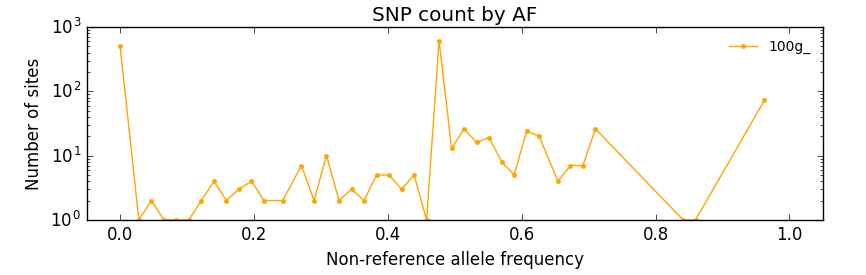
\includegraphics[type=pdf,ext=.pdf,read=.pdf,width=23cm]{100g-counts_by_af.snps}\\%
\noindent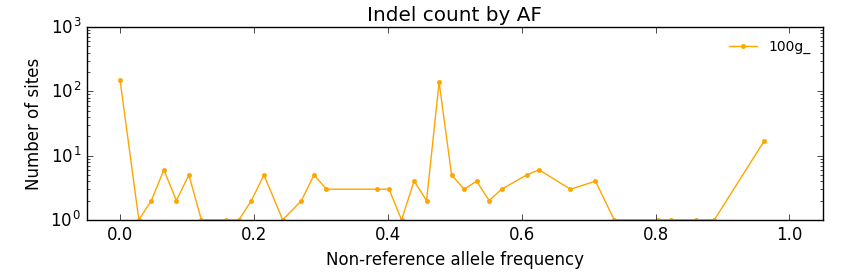
\includegraphics[type=pdf,ext=.pdf,read=.pdf,width=23cm]{100g-counts_by_af.indels}}}

% Ts/Tv by AF
%
\hslide{Ts/Tv by AF}{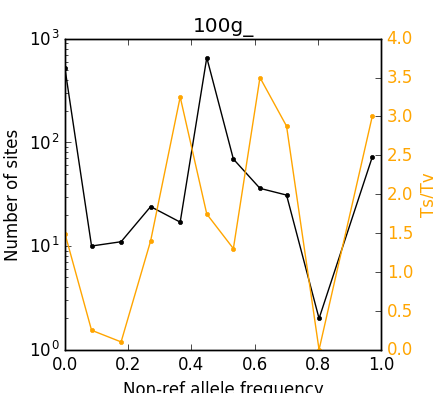
\includegraphics[type=pdf,ext=.pdf,read=.pdf,width=15cm]{100g-tstv_by_af.0}}

% Ts/Tv stratified by QUAL
%
\hslide{Ts/Tv stratified by QUAL}{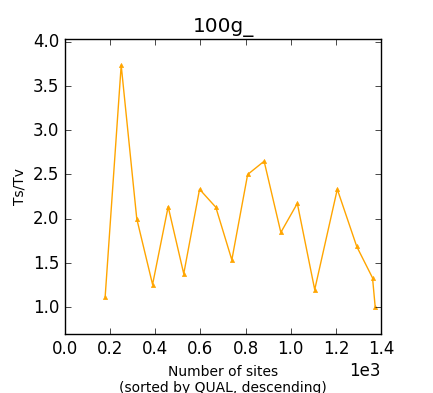
\includegraphics[type=pdf,ext=.pdf,read=.pdf,width=15cm]{100g-tstv_by_qual.0}}

% Indel distribution
%
\hslide{Indel distribution}{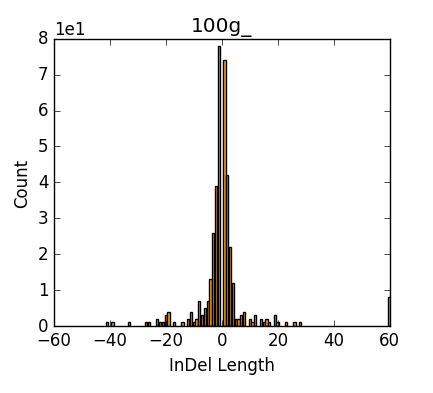
\includegraphics[type=pdf,ext=.pdf,read=.pdf,width=15cm]{100g-indels.0}}

% Depth distribution
%
\hslide{Depth distribution}{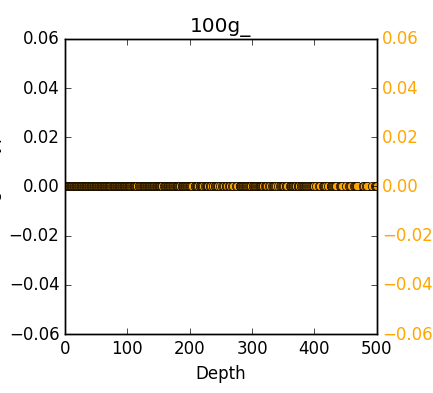
\includegraphics[type=pdf,ext=.pdf,read=.pdf,width=15cm]{100g-depth.0}}

% Substitution types
%
\hslide{Substitution types}{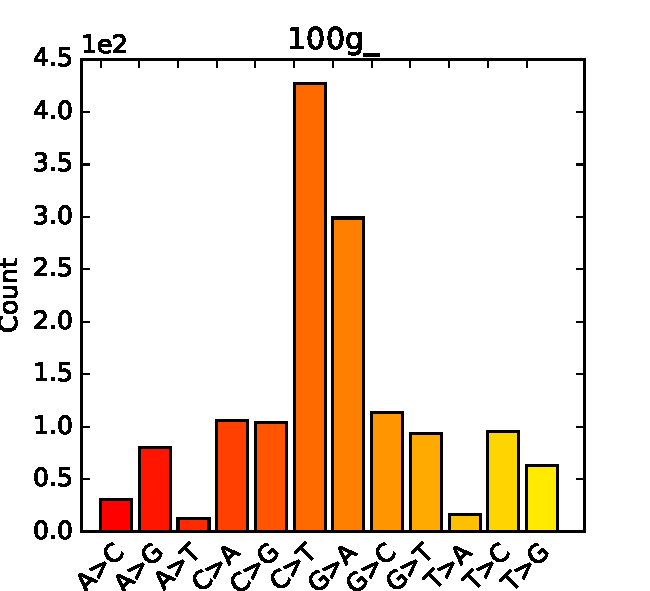
\includegraphics[type=pdf,ext=.pdf,read=.pdf,width=15cm]{100g-substitutions.0}}


\end{document}
